\documentclass[a4paper, 11pt, twocolumn, twoside]{report}
\usepackage[utf8]{inputenc}
\usepackage[a4paper,width=150mm,top=25mm,bottom=25mm,bindingoffset=6mm]{geometry}
\usepackage{natbib}
\usepackage{graphicx}
\usepackage{fancyhdr}
\usepackage{titlesec}
\usepackage{todonotes}
\PassOptionsToPackage{hyphens}{url}\usepackage{hyperref}
\usepackage{enumitem}
\usepackage{graphicx}
\usepackage{hyperref}
\graphicspath{ {img/} }

\newcommand{\chapfnt}{\fontsize{16}{19}}
\newcommand{\secfnt}{\fontsize{14}{17}}
\newcommand{\ssecfnt}{\fontsize{12}{14}}

\titleformat{\chapter}[display]
{\normalfont\chapfnt\bfseries}{\chaptertitlename\ \thechapter}{20pt}{\chapfnt}

\titleformat{\section}
{\normalfont\secfnt\bfseries}{\thesection}{1em}{}

\titleformat{\subsection}
{\normalfont\ssecfnt\bfseries}{\thesubsection}{1em}{}

\titlespacing*{\chapter} {0pt}{50pt}{40pt}
\titlespacing*{\section} {0pt}{3.5ex plus 1ex minus .2ex}{2.3ex plus .2ex}
\titlespacing*{\subsection} {0pt}{3.25ex plus 1ex minus .2ex}{1.5ex plus .2ex}
\titlespacing*{\subsubsection} {0pt}{1.5ex plus 1ex minus .2ex}{1.0ex plus .2ex}

\pagestyle{fancy}

\fancyhead{}
\fancyhead[RO,LE]{Membrane - Distributed File Backup}
\fancyfoot{}
\fancyfoot[LE,RO]{\thepage}
\fancyfoot[LO,CE]{Chapter \thechapter}
\fancyfoot[CO,RE]{Dominic Hauton}

\graphicspath{ {img/} }

\bibliographystyle{agsm}

\setcitestyle{square}

%opening
\title{Membrane - Distributed File Backup}
\author{Dominic Hauton}

\begin{document}

\maketitle

% Copyright and declaration

\begin{abstract}
An application in which users can join a large public network of intelligent storage agents to trade their available file space. This will allow the user to backup and version files safely on potentially untrustworthy computers, increasing availability and redundancy. The hosts will act as intelligent agents, and trade space when they communicate with one another.
\end{abstract}

\renewcommand{\abstractname}{Declaration}
\begin{abstract}
\hfil I declare that... \hfil
\end{abstract}

\renewcommand{\abstractname}{Acknowledgements}
\begin{abstract}
\hfil With thanks to my supervisor, Russell Bradford \hfil
\end{abstract}

\tableofcontents

\chapter{Introduction}
Distributed storage is a well studied and explored domain with clear advantages over storage on a single machine. In order to implement a peer-to-peer distributed agent based storage system we must first decompose the problem into several parts and explore the advances made in those fields as well as looking at advantages of existing technologies.

\section{Project Goals}

The goal of Membrane is to allow users to easily backup and recover the contents of folders on their computer without needing to pay for a subscription-based service. Looking at breadth of products available it quickly becomes evident that there is a huge desire for external backup, and many people now take popular cloud storage services such as Dropbox and Google Drive for granted. \citep{dropbox2015popularity}

To make Membrane competitive with existing solutions we must aim for two important features, ease of use and the ability to access your files from any system provided you can log into your account. On a centralised backup system this a trivial task, however, with a distributed system the concept of creating an account, logging in, finding peers and discovering which users hold your files is a much greater challenge.

In this project we are working towards a proof of concept of the idea of distributed backup, creating the fundamentals of the Membrane, focusing on the key aspects of distributed storage, but we will leave certain convenience features out for later development if the project proves successful. This is consistent with the Minimum Feature Set methodology described by \cite{blank2010mfs}, a practise which is now used heavily amongst technology startups. The technique aims to reduce engineering hours and get the hands in the product of early visionary users early to encourage feedback.

The first step of the project will involve looking at existing products, seeing what design lessons from them we can apply to Membrane. We will then approach potential users and inquire what features they think are important in a system such as Membrane. A technology survey will be performed to assess what technologies we can use to ease with development, the solution will be built, and tested by users, whose feedback we will incorporate in the final prototype.

\section{Need for Membrane}

With the advent of cheap high-speed internet users are now able to use monolithic cloud services to backup data. These tend to be expensive for anything but small amounts of storage and many people have expressed security concerns over holding their data in a data centre owned by another company. \citep{batters2010dbsecurity} Especially if their data leaves the users country where data protection laws may be different.

Over time personal storage capacities for users have also increased. It is now common for computers to come with large amounts of hard drive space which is often not filled to capacity. The project proposed promises to swap this free hard drive space to back up other users’ data in exchange for their surplus space to backup your data.

To simplify the process, the system will be able to negotiate contracts of varying complexity for space allocation on another machine, in exchange for space on itself. Unlike most distributed databases and cloud storage solutions frequent down-time will be expected across devices and contracts will have to account for this.

There is an open gap in the market for a distributed storage solution which focuses entirely on backup and trading data, rather than charging a fee for storing data. The users of Membrane would be able to benefit from the advantages of commercial services, without any of the previous highlighted downsides.

\section{Challenges}
There are multiple challenges associated with creating both decentralised systems and backup solutions.

While doing this it is important to keep resource usage down as Membrane is a background process and should not be notice by the user. To achieve this we need to explore methods of reducing bandwidth, memory and processor usage.

As part of this we need to find a way to copy the minimum amount of data required during backups, an effective way of managing where file chunks are stored, a way to encrypt the files on the remote host and a way to periodically authenticate that the host still holds the file.

Part of the required research also includes exploring the more recent technology of intelligent agents, in which we are most interested in trust metrics. Intelligent agents will allow the software to make storage decisions based on the trust and reputation of other nodes in the network that it has interacted with in the past.

\section{Modules}

Membrane will be built up of several predetermined modules performing distinct roles. This have been broadly identified at this stage as a guide for our literature review and for technology decisions.

The core of any backup system is the file system watcher that determines whether a file has been modified, added or removed. This must be able to cheaply assess if a file or folder has changed and determine whether the altered file needs to to be refreshed in the storage system.

Once a modified file has been detected that change needs to be catalogued and the bits required to restore the file must be stored locally for further processing. This causes temporary duplication, however this must be performed so modification to the real files can continue while a peer willing to store the file is located. This system must also be able to recreate the file from the bits stored.

Next a system needs to be put in place to package bits from various files into a block of data that a peer can store. This system needs to be able to determine which peer certain bits should be stored with and how many peers the file should be stored with, based on trust, availability and other useful metrics that will be explored.

Finally a module responsible for networking and authentication must be created. This must be able to authenticate the user, find peers, establish connections to new peers and deal with the challenges to creating a secure communication link to the peers.

\section{Conclusion}

We have established the need for Membrane and briefly covered the advantages compared to existing solutions. We have also discussed the basic structure of Membrane and what challenges we expect to face during development. We will explore these further in our literature review.

\chapter{Literature Review}

The literature review aims to preempt challenges by finding solutions to similar problems in literature and existing pieces of software.

We will first explore the history of file backup, proceeding into the challenge of locating, trusting, connecting and communicating with peers. Finally we will look at authentication issues as well as exploring how a peer can prove they own a file, without re-sending the entire file back to us.

\section{History of Problem}

A simple file backup can be imagined as simply copying a file to another location. In order to keep the duplicated file in sync they must be compared. The program diff solves this through finding the longest common sub-sequence of bytes between files. In order to improve performance hashing, presorting into equivalence classes, merging by binary search, and dynamic storage allocation are used. \citep{hunt1976algorithm}. This allows the user to view changes and copy the file over again if required.

\subsection{Rsync}
In a networked scenario, bandwidth from source to destination is at a premium. Rsync, introduced in 1996 presents a much better solution through copying changed file chunks (deltas). \citep{tridgell1996rsync}. Rsync splits the file into shards and calculates a weak rolling checksum and strong MD4 checksum for each block that allows quick comparisons of shards along the file. When a discrepancy is found, we assume an extra byte or bytes have been added to the file. The weak checksum can be efficiency recalculated for the next offset and once there is a match, it is confirmed with the strong checksum. The new added chunk can now be transmitted. This results in a lot less data being copied than there would be with a diff file. \citep{tridgell1996rsync} This combination of weak and strong check-sums has been used across multiple distributed systems including low-bandwidth file systems \citep{muthitacharoen2001low} and high performance transactional object stores. \citep{stephen2000platypus}.

Multiround Rsync improves on the rsync algorithm by allowing for more communication to lower bandwidth. Blocks of smaller and smaller sized are used to find holes in the old file in each round and the file until the minimum block size is reached and a copy occurs. \citep{multiroundrsync} This works better than standard rsync in situations where the source file has been changed in many places distributed around the file.

Rsync requires both old and new copies of a file to exist on the host system during an update. This issue has been addressed by creating an in-place rsync (ip-rsync) that uses techniques used in delta compression and Lempel-Ziv compression to move the areas of the file around. In ip-rsync file sender sends add and move commands to the destination in an order that guarantees no files will be overwritten. \citep{rasch2003place}


\subsection{Git}
Git is an improvement on Rsync as it provides both version history and minimises data transfer. To keep storage simple, a copy of the whole file is stored and a reference is put into the version history. By storing old files locally operations are fast. This is also an important distinction from other version control systems and one of the reasons why Git was chosen as an example versioning system compared to other versioning systems like SVN. The systems can continue to operate without a centralised server. To reduce file duplication all files are referenced using their SHA-1 hash. This means you can be sure the contents of the file hasn’t changed since you last read it. \citep{torvalds2010git}

Git also uses a 3 stage workflow. A working directory, where the current files are stored, a staging area and a .git directory. The staging area prepares your next commit and then it is finally committed. When the staging is complete the change is irreversibly stored. This is a good approach that will be adopted in the final software solution. It will allow incrementally finding changed files, and assessing the need for a new version number to be saved.


\subsection{Bittorrent}
The BitTorrent protocol is a mechanism for sharing files between swarms of hosts. As BitTorrent splits files into parts, users start sharing data even before they have received the full file. Each file has a SHA-1 identifier, similar to Git. \citep{qiu2004modeling}

If a user wishes to download a file from the swarm, the user downloads a metadata file from the web and locates users sharing the data using a Tracker Server, Distributed Hash Table (DHT) or Peer Exchange (PEX). \citep{cohen2008bittorrent}

A Tracker server is a centralised store of all current connected users along with how much of the file they hold. This approach is vulnerable to exploitation by authorities as all of the data about a swarm is stored on a single server and as a result cannot be used for the proposed system.

A DHT contacts other known users for information instead of a centralised server. The Mainline DHT as outlined in BEP No.5 is based on the Kademlia protocol that allows for decentralised peer discovery for a particular piece of content.

PEX is a method for two clients to share a subset of their peer lists. Coupled with DHT, PEX removes a vulnerability from the Bittorrent network by allowing fully distributed bootstrapping, tracking and peer discovery.

A DHT with a form of PEX a tried and tested way of successfully mapping and finding files on a network and will be used within the proposed project.

\subsection{Resilio}
Resilio Sync is an example of a distributed file storage system that utilises the BitTorrent protocol to automatically synchronise folders between a user’s systems. It is not a cloud backup solution and not intended as a form of off-site storage. There is no distributed file system and as a result, no redundant data block algorithm adding complexity. \citep{farina2014bittorrent}

As Resilio Sync uses DHT to transfer data, there is no central authority to manage authentication or log data access attempts. This makes it difficult to determine whether a file has been accessed by another user. \citep{farina2014bittorrent} As a result in the project the assumption will be made that everyone in the network has access to all encrypted file chunks. To access and reassemble a file, a user will be required to request all of the file chunks individually and then locally reassemble them.

\subsection{Storj}
Storj is a peer-to-peer cloud storage network which aims to allow users to store files on a decentralised platform. The platform takes special care to provide protection against Sybil attacks and other forms of fraud. \citep{Wilkinson14storja}. To store files it stores encrypted hashed shards on the network. In order to provide proof of storage it uses Merkle Audits and pre-generated audits with hash-challenges to determine whether the client still holds the required data. By adding a seed to the hash-calculation the client can enforce the workers are still in possession of the data. It prevents the client cheating a farmer through using blockchain proof-of-existence to keep both parties honest.

The most efficient form for proof of storage is through using a deterministic heartbeat. Using Feistel permutations data can be verified with $n + 2 \sqrt{n}$ challenges. Erasure encoding is added to shards to detect any minor changes to the data. This is less I/O intensive than a full heartbeat, but still allows an attacker to complete heartbeats with only a data integrity of 1/n, where n is the number of nodes holding the data.

In order to add extra protection to files, we can use erasure encoding to allow file recovery if one of our shard types is lost. This can be investigated in our software, however, as the shards are expected to change on a regular basis because of versioning, this may not be possible.

To prevent Sybil based attacks, Storj encrypts each shard segment with a different salt. This stops workers completing proof of storage on behalf of another node.

\section{Peer Admission}
The first step in designing the distributed file system is locating other peers within the swarm. This is accomplished through Peer Admission. Once the first peer is found data within the swarm can be located using a DHT which guarantees content can always be found.

\subsection{Bootstrapping}

There are two types of PTP networks which must be examined:
\begin{itemize}
 \item \emph{Asynchronous}
 \item \emph{Synchronous}
\end{itemize}

Within Synchronous networks the number of nodes on the network is constant and all of the nodes are aware of each others existence. This does not allow storage networks to scale but it does allow data to be kept private. \citep{saxena2003admission} This is the simplest and first approach that will be taken in locating nodes within Membrane.

In most current P2P systems such as Gnutella \citep{klingberg2002gnutella}, Chord and Tapestry as well cryptocurrencies such as in Bitcoin and Litecoin a bootstrapping node is contacted, which provides information about what clients are currently online. Once a bootstrapping node allows the client to find the edge of the swarm, more information can be found using peer exchange.

Within a local network we can also use Universal Plug and Play to find other nodes within the local network. This prevents an external call to a bootstrapping node and as a result is less prone to attack.

Through looking at availability metrics within Bittorrent systems \cite{neglia2007availability} determined that both trackers and DHT should be used in creating a highly available distributed storage system such as BitTorrent. DHT tends to be slower at finding new data, however it is much more reliable.

Within Membrane, I plan to use a combination of Asynchronous and Synchronous techniques. Users will try to bootstrap from their last known neighbour nodes on the network, this takes advantage of the static nature of the backup data. Only if this fails, and with the user's permission will they contact a centralised bootstrapping node. This should only happen during a first install and if the user has no referrals. Throughout the lifetime of the application the centralised bootstrapping node would ideally be replaced with a referral system.

A further extension of this, would be to allow hosts to provide a DNS name along with their IP. Users that have setup Dynamic DNS (DDNS) \citep{bound1997dynamic} would be able to locate each other without the help of a bootstrapping server.

\subsection{Peer Exchange}

When bootstrapping is complete new Peers can increase their knowledge of the network through Peer Exchange. This is used by Bittorrent to help share swarm information with other nodes. As soon as a client connects to the swarm, peer information is collected using DHT or PEX.

There are two common extension protocols called AZMP and LTEP, which send at most one message a minute when a client leaves or exits the swarm. To reduce congestion at most 50 peers can be added or removed in one PEX message. \citep{vuze2010vuze}

\subsection{Shard Discovery}

Bittorrent also uses the Mainline DHT to find other hosts in the network. This is a Kademlia DHT which now according to \cite{jones2015mainlinedht}, now supports 25M users. It works through assigning each node and file a 160-bit string as an ID. We can work out which node is meant to store a file metadata and crawl in the direction of the node using a hill climb algorithm. Once the metadata is stored on the host, if a host host wants to download a file, it can take the metadata on the known host to find the IP of hosts with the file.

Hosts in Membrane will store a metadata file with all of the information required for the specific account to run, including friends, encryption keys as well as local mappings for which host owns which shard and which IP belongs to each host. As a result a DHT will only be required if this initial metadata is lost and needs to be recovered. The proposed version of Membrane will make use of this metadata, but recovery can be added in further iterations of the project.

\subsection{Dynamic IP Address}

Dynamic IP addresses have proven to be problematic in distributed computing, as ISP typically charge more for users to have a static, unchanging IP. Bittorrent tackles this issue through using a DHT to dynamically find the IP address of the user that owns a file. This approach is robust, however, it is a complex solution to IP address resolution.

Another widely used approach is using Dynamic DNS (DynDNS) as described by \cite{bound1997dynamic} in RFC 2136. This allows a client to automatically update a nameserver with a new IP or other information, this allows clients to have a persistent addressing method for devices that change their location. This approach requires initial configuration by the user, however, it provides a reliable way to connect with a user when their IP is lost. There are several tools such as MintDNS, cURL and Iandyn that could be used to ease the development of a built in DynDNS. When setting up a relationship with another host, both an A/AAAA Address and CNAME could be provided, where the CNAME is a backup if the A/AAAA address does not work.

To resolve IP Address resolution within Membrane, I would like to take advantage of small-world networks. \citep{porter2012small}, in which the mean shortest-path between two nodes increases slowly compared to the number of notes in a network. Within a group of users in Membrane hosts are likely to share multiple first, second and third degree connections. By storing a list of IP addresses from all of the hosts. It is highly unlikely that all connections within three hops will have changed IP address. We take inspiration from ARP \citep{plummer1982ethernet}, and send broadcasts with a limited hop count in the network to see if anyone is aware of the current address of a host. The downside of this approach is that it relies on a node within your social network to be online. Measures will need to be put in place to reduce broadcast spam.

A broadcast storms runaway broadcast events, common in networks that used broadcasting for communication, particularly when areas of the network overlap. \citep{Tseng:2002:BSP:506900.506905} These can be mitigated by reducing broadcast traffic, however, Membrane will rely on broadcasts to find hosts. The first step to limiting these broadcasts, is implementing a hop count on broadcasts. This is commonly seen in routing protocols such as IPv6 \citep{deering1998internet}. The Spanning Tree Protocol (STP) as seen in IEEE 802.1d \citep*{ieee802ieee, sharma2004viking} provides loop-free routing in LANs by pruning redundant links. Topology changes are dealt with by rebuilding the tree.

Within Membrane rebuilding a Spanning Tree would be an expensive operation. If broadcasts become a problem a 'block request' system can be used, similar to that of ICMP redirects. \citep{postel1981rfc} If a node receives a duplicate broadcast message it sends a request back one hop to not send broadcasts from that source toward it for  some time. The time limit would allow allow for corrections if the network topology changes. This preventative approach and could be improved by using the full Spanning Tree implementation. As a further step it could be improved by using a DHT 'closest jump' approach if required.

\section{Data Allocation on External Nodes}

In order to store data on another node Membrane must first have permission to store files on another node. In order to make a choice we must be able to look at trust information about other nodes on the network, and negotiate and trade space once a suitable candidate has been found. These two areas have been explored in the context of Multiagent Systems (MAS) in the past. \citep{wooldridge2009introduction}

\subsection{Negotiation}

Negotiation aims to reach a level of resource allocation that is acceptable for all involved parties. \citep{rahwan2005interest} It allows two or more parties that value each others service, to participate in a mutually beneficial exchange of services, however, as there are multiple beneficial outcomes it can be defined as "distributed search through a potential space of agreements" \citep{jennings2001automated} Within Membrane, this service is storage space, that is physically separated from the current user. We now take a look at negotiation and how we can build a negotiation framework that our agents can use to exchange storage.

There are three main areas that are important for negotiation. Negotiation protocols, negotiation objects and the node's reasoning models. \citep{beer1999negotiation} The sophistication of the negotiation is determined by each of these and can take different forms such as auctions, argumentation and protocols in the style of a contract net. The simplest negotiation uses fixed size items, which Membrane shall be initially using for this reason. More complex negotiation allows for counter offers and stronger guarantees.

A simple negotiation protocol issues a call for proposals to a number of nodes and waits for their bids. To formalise this a Agent Communication Language (ACL) such as KQML (Knowledge Query and Manipulation Language) \citep{finin1992specification} or the more modern FIPA (Foundation for Intelligent Physical Agents) \citep{fipa2002fipa}. \citep{rahwan2005interest} \cite{beer1999negotiation} tells us that within KQML the agent sending the query is expected to decide how the receiver will handle it, which places limits on negotiation. On the other hand, FIPA is newer and as a result can be more error prone.

\subsection{Negotiation Logic}

The form of negotiation within Membrane also needs to be decided. We must first decide on a reasoning mechanism to use within the agent. The distinction between monotonic and non-monotonic logic is important in the study of AI and multiagent systems. In non-monotonic logic new axioms (or knowledge) can invalidate old theorems. \citep*{mcdermott1980non, antonelli2008non} This is important in the real world as we need to be able to make assumptions on facts and retain flexibility in our understanding of the world. Within a MAS a non-monotonic logic can be more difficult to implement as theorems need to be constantly asserted, and as a result they often result to first-order (or monotonic) logic. Within Membrane we need to implement a monotonic logic to assert trust in our contracts and negotiations. In the context of a negotiated contract, throughout it's duration, we cannot effort to re-evaluate our trust of the agent.

\subsection{Negotiation Tactics}

In order to exchange storage space we must find the most suitable node in the network. There are multiple negotiation tactics between agents for collaboration and coming to an agreement. \citep{beer1999negotiation} We shall explore the advantages and disadvantages of game-theoretic approaches \citep*{rosenschein1994rules, kraus2001strategic, sandholm2002algorithm}, heuristic-based approaches \citep*{faratin2000automated, fatima2002multi} and argumentation-based approaches \citep*{kraus1998reaching, jennings1998argumentation} as well as exploring practical implementations negotiation. Ideally a negotiation mechanism is computationally cheap, produces good outcomes, distributed, fair to all participants, compatible with fixed strategies and is able to function without complete information. \citep{rahwan2005interest}

Using a \emph{game theory} approach we assume all agents are self-interested and allows agents to analyse optimal behaviour. \citep{osborne1994course} We can apply this in agent reasoning by giving each combination of collaborations a utility. Doing this an optimal set of interactions can be calculated. This can even be used to help agents interact in a certain way. \citep{varian1995economic}. The main downsides include the assumption of unbounded computational resources, complete knowledge of the outcome space. \citep{rahwan2005interest} This makes a game theory approach unusable in Membrane as the network is not fully understood by each agent.

A \emph{heuristic} approach produces 'good enough' negotiations. Instead of exploring the full extent of possibilities they focus on the subset most likely to lead to positive interactions. In the context of Membrane, this may be hosts that you have had successful interactions with before. The downsides of this approach is that it becomes difficult to predict the negotiation actions of other agents and as the full search space is not explored the result may not be optimal. \citep{jennings2001automated}

A \emph{argumentation} approach is beneficial when a flexible negotiation is required and the agents have limited knowledge of the world. It's commonly used in the human world by advertisers to convince humans to try products. \citep{slade2002reasons}. Instead of simply rejecting an offer a agent can say why or offer a counter-proposal, which can result in more successful negotiations. Although this approach offers far better negotiation, it is much more complex to implement and is not required within initial implementations of Membrane.

\subsection{Practical Negotiation}

We now look at practical real-world negotiation. Real world approaches take into consideration the practical implications of reasoning systems and prove that concepts work. Within cloud computing an agent is often required to request a service. The use of these resources is based on service-level agreements (SLAs) which are designed to provide users with a service when requested. \citep{paletta2009mas} One critical issue in SLAs determining the  Quality of Service (QoS) constraints of the offered service.

\cite{yan2007autonomous} explores creating a SLA negotiation system, splitting SLA negotiation into three parts. Defining \emph{Negotiation Protocol} that allows participants to send offers to each other, \emph{Negotiation Coordination} which ensures the final result of the negotiation fulfils the QoS requirements of the agent and a \emph{Decision Making Model} which allows the parties to decide if they are satisfied with the deal.

Within Membrane, hosts are unable to know if they will be compatible with another agent. It might be the case that they both have 50\% uptime, however they are never online at the same time. As a result a system will have to be created to allow agents to find if they are compatible with each other and storage decisions will have to be based on this.

\cite{paletta2009mas} presents an negotiation mechanism which makes use of mean algorithm and protocol, using key awareness concepts first proposed by \cite{herrero2007agents}. It uses an quantitative metric in the range [0, 1] to decide how much the agent should be collaborating with another agent. The agents can then communicate using the messages:

\begin{enumerate}
 \item REQUEST - Can you perform A?
 \item CONFIRM - Yes I will do A.
 \item DISCONFIRM - No I will not do A.
\end{enumerate}

Collaboration decisions decided using an Artificial Neural Network (ANN). Three metrics are used, physical resource availability, if the node is available for collaboration and the number of previous collaborations of the same type. The ANN used was a Multi-Layer Perceptrons (MLPs) using one hidden layer and two units.

When evaluated the mechanism was able to deal with 93\% of situations and negotiation with the first node was successful 68\% of times. \citep{herrero2007agents}

With Membrane we take this model and make it more practical by introducing reputation to allow third party ratings to be shared.

\subsection{Service Level Agreements}

In order to create a negotiation system we need to explore what makes up an successful software SLA. \cite{keller2002defining} defines the WSLA framework which sets out to create a SLA based negotiation frame work.
They describes 3 key areas that must be present in an SLA.
\begin{enumerate}
 \item Parties Involved
 \item Service Description
 \item Obligation
\end{enumerate}
Within Membrane the parties involved will always be the two nodes exchanging information. The service description will be a promise to store a block of data on another host. The obligation will include various parts such as proof of storage and the ability to update and retrieve the data a set number of times. These will be explored when the SLAs for membrane is designed.

Another key area \cite{keller2002defining} discusses is the 5 stages of an SLA lifecycle.
\begin{enumerate}
 \item SLA Negotiation and Establishment
 \item SLA Deployment
 \item Measurement and Reporting
 \item Corrective Management Actions (in case of violation)
 \item SLA Termination (in case of violation)
\end{enumerate}
These are the backbone of every real SLA and will be explored in more detail while designing the negotiation system for Membrane.

\section{Trust and Reputation}

Agents in a distributed system need to be able to protect themselves from 'bad' agents. \cite{pinyol2013computational} describes three main approaches to control the acts of agents. The \emph{Security Approach} which guarantees the authenticity and integrity of interactions. The \emph{Institutional approach} which relies on a central authority to enforce good behaviour and finally the \emph{Social approach} which allows agents themselves to punish other agent for 'bad' behaviour. This final approach is where trust and reputation is used.

Trust can be used to predict the behaviour of an agent. \citep{wooldridge2009introduction} A classification presented by \cite{balke2009using} defines 5 stages that exist in reputation and trust models. Co-operative behaviour is first stored and then rated using a utility function. Within Membrane it is easy to see the utility being rated as shared transaction time. This cooperative behaviour is then stored in an image of the other agent at a predetermined level of detail. This image can now be recalled to infer trust. Finally the agent can use this trust to learn and adapt it's strategy.

The ReGreT model \citep{sabater2001regret} is ``one of the most complete reputation and trust models'' \citep{pinyol2013computational} so we shall use it to see what a good trust system includes. It uses direct experience, third party information and social structures to calculate trust, reputation and credibility of another agent. An important note for this model is that trust is contextual. Agent a will trust b while certain conditions are met. In the context of Membrane, perhaps another agent will refuse to return our data, if we cannot prove that we still have their data, which would mean that they would be useless if the client experienced completed data loss. We must therefore consider simulating a situation in which complete data loss was experienced.

\subsection{Trust and Reputation Attacks}

Attempts to misrepresent reliability and manipulate reputation are common in traditional communities and have been exploited by con artists for centuries. In a distributed system agents must be able to protect themselves against common trust attacks. \cite{josang2009challenges} describes 9 potential attacks on reputation systems.
\begin{itemize}
 \item Playbooks - Gain high reputation and burn it quickly with low quality actions
 \item Unfair ratings - Give incorrect reputation or image
 \item Discrimination - Give high quality service to one set of users and low quality to another set
 \item Collusion - A coordinated reputation attack.
 \item Proliferation - Offer a service through multiple channels
 \item Reputation Lag Exploitation - Provide a large number of low-quality services quickly
 \item Reentry - Change identity to recover reputation
 \item Value Imbalance Exploitation - Gain reputation with easy actions
 \item Sybil Attack - Inflate reputation with fake accounts.
\end{itemize}
When implementing a trust system in Membrane these attacks should be considered and special attention should be paid to prevent a new user being exploited for their storage space when joining the swarm.

\section{Communication}

As Membrane is a distributed system communication is key for nodes on the network to interact. It is traditional to form a protocol that agents can use to share information with each other. These protocols are often very rigid and do not allow for expansion. Formalising communication using ACLs is a more flexible approach that aims to let agent share a common understanding of the domain, and allows hosts to reason about communication themselves. Instead of using a strict protocol we shall instead take an agent-based approach to communication using ACLs.

\subsection{Agent Communication Language}

On balance, we shall be using FIPA for communication. This is an ACL based on Speech Act Theory \citep{labrou1999agent}. It splits communication into a communicative act (CA), an ACL message structure and a set of communication protocols such as XML or OWL (Web Ontology Language). In FIPA communication should be rational, in that when sending a message:
\begin{itemize}
  \item The sender believes the proposition.
  \item The recipient does not already believe the proposition.
  \item The recipient will believe the proposition after the proposition.
\end{itemize}
In the case of Membrane this could be put into the context of asking another node to store data, it would only be reasonable to send another node data to be stored, if the two nodes had negotiated storage of that block between them previously.

To keep communication simple for nodes, we shall use two CAs
\begin{itemize}
  \item REQUEST
  \item INFORM
\end{itemize}
where \emph{REQUEST} expects a reply of some sort and \emph{INFORM} does not. This will enable easier implementation and can be expanded if required.

\subsection{Ontology}

An ontology is a way of defining basic terms and relations comprising the vocabulary of a topic area. \cite{sugumaran2002ontologies} tells us the the three most commonly used relationships in an ontology are \emph{is-a}, \emph{synonym} and \emph{related-to} (which is a generic association between entities). So why should we create an ontology for membrane? \cite{noy2001ontology} lists the benefits of ontology within distributed systems:
\begin{itemize}
 \item Enable common understanding of the structure of information
 \item Enable reuse of domain knowledge
 \item Make domain assumptions explicit
 \item Separate domain and operational knowledge
 \item Analyse domain knowledge
\end{itemize}
Within Membrane we could benefit from an ontology during negotiation for storage space. Obligations could be predefined between agents and an agent could request a set of obligations, instead of explaining an obligation during negotiation. This allows agents to be more concise and expressive. \cite{noy2001ontology} gives us 7 steps for ontology creation.

\begin{enumerate}
 \item Determine the domain and scope of the ontology
 \item Consider reusing existing ontologies
 \item Enumerate important terms
 \item Define classes and their hierarchy
 \item Define class properties (slots)
 \item Define slot facets
 \item Create Instance
\end{enumerate}

It is important to ensure the ontology goes into the right amount of detail for the requirements. An overly detailed ontology can make reasoning difficult, and an ontology that is too simple will limit expressiveness and reasoning. \citep*{wooldridge2009introduction, sugumaran2002ontologies}.

When considering ontologies for re-use \cite{noy2001ontology} points us towards the DAML ontology library (http://www.daml.org/ontologies/). Using this and Google I was able to locate 2 ontologies, the datastore schema provided by \cite{w32001datastore} and an OWL based ontology for SLA services provided by \cite{pande2012slaont}. Both of these will be examined further during the ontology creation process.

\section{Peer-to-Peer Connection}

Network Address Translation (NAT), defined in RFC 2663 by \cite{srisuresh1999ip} is used extensively to solve the IP exhaustion problem, however, it also creates a lot of well documented problems for peer-to-peer communication as the IP address a hosts has set, may be a private and only useful for peers on the same network. Multiple Membrane hosts may be using the same IP address and the TCP listening port used by a node will change between connections. In order to transfer data over NAT a NAT-Traversal Technique must be employed. There are four major techniques described by \cite{ford2005peer} that we shall explore.

\emph{Relaying} is a method of communicating through a well known server, that has a static IP address and port. This has the advantage of being simple, however, it has the disadvantage of using the server's processing power, network bandwidth and increases latency between peers. It is a good fallback strategy but also requires both clients to initiate the connection, which makes listening for incoming connections difficult. The TURN protocol \citep{rosenberg2005traversal} describes a fairly secure method for relaying.

\emph{Connection Reversal} is the use of an external server to request a 'call back' to a host. The connecting host contacts an external server with a target host and leaves it's public IP and port. The relaying host can then choose to send a request to host behind NAT and the host behind NAT can choose to forward the request. It has similar limitations to relaying, however, it is easy to imagine an implementation that uses connection reversal for bootstrapping a P2P connection.

\emph{UDP Hole Punching} is a technique defined in RFC 3027 5.1 \citep{holdrege2001rfc} that allows two clients behind NAT to connect with the use of a rendezvous (RV) server. Hosts contact the RV and leave their UDP port and address. You should be weary of poor NAT implementations translating IP addresses within data when packets are coming in and out. \citep{ford2005peer} When clients are both behind the same NAT, packets between them do not need to go through NAT. If Hairpin NAT is correctly configured they will be bounced back within the internal network, however, it could result in overheads otherwise. If this problem is detected during the implementation of Membrane private IP address could also be sent to the RV server. It's important to consider that the ports behind a NAT are dynamically allocated, so connections must be authenticated between connections, to ensure the IP address and port still direct towards the same host. The initial outbound packet from a host to a the RV server is key in 'punching a hole' through the NAT. The timeout of a hole punched port can be as low as 20 seconds, so the host must maintain the hole by sending single packets to the RV on a regular basis.

\emph{TCP Hole Punching} is more complex than with UDP as clients need to establish sessions across the NAT. For hole punching to work the same port needs to be used for listening and establishing a connection. This can be done using \emph{SO\_REUSEPORT} option, which allows an application to claim multiple sockets from the same endpoint. Within the application an new port needs to used for handling the connection.

There are two practical solutions that I shall explore for implementation within Membrane. TURN \citep{wing2010traversal} provides a set of methods for NAT hole punching. UPnP \citep{boucadair2013universal} is a method through which a host can request a NAT gateways to open a port for the application. There have been security concerns with UPnP which has resulted in UPnP being disabled on many routers. This will need to be explored during implementation of Membrane.

\section{Distributed File System}

Membrane shards files and stores copies on multiple nodes for redundancy. This is a technique that is commonly found in distributed file systems (DFS) such as Hadoop File System (HDFS) \citep{hdfsAnalysis}, Google File System (GFS) \citep{TheGFS} and Parallel Virtual File System (PVFS) \citep{ross2000pvfs}. This section aims to explore the reasoning and decisions taken with these file systems.

HDFS has proved to be highly successful in storing large quantities of data over thousands of nodes and is used by over 100 organisations world wide. It stores file system metadata on a central dedicated server called a NameNode \citep{hdfsAnalysis}. This is a similar approach to GFS \citep{mckusick2010gfs}. Membrane takes this approach by storing file metadata on the client. Ceph takes this approach further, storing file meta on a distributed cluster of NameNodes, using hash function to spread metadata over the name nodes. \citep{weil2006ceph} This allows for larger, more distributed system, this could be used within Membrane if meta-data proves too large to store on the client.

Files and directories are represented my inodes, these record attributes such as permissions and location. Within Membrane this will need to store information such as checksums, encryption keys and SLA for each file, to allow each file to be verified on a regular basis. When writing data to the cluster the NameNode chooses the targets for shards. The client in Membrane will be able to negotiate shard targets on the network using mechanisms described previously.

The NameNode stores the metadata as a combination of a checkpoint and journal (a write-ahead commit log). If there is a fault on the NameNode, such as a power outage, the journal can be replayed over the latest checkpoint. In HDFS a new snapshot is created during a node restart, however, in Membrane the journal is kept to be able to restore the metadata during any point in the journal. By not removing any shard that is still in the journal we are able to rollback to any previous state in ahead of the oldest checkpoint.

In HDFS, during startup a DataNode connects to a NameNode, and performs a handshake with a unique storage ID that can identify it. In addition a DataNode will also send heartbeats and reports on a regular basis. \cite{hdfsAnalysis} This is a great approach as it makes the DataNode responsible for notifying the NameNode that it still holds the data. Not the other way around. A similar approach will be used in Membrane, however, the NameNode will also request some proof that the DataNode still holds the file, as in Storj.

In both GFS and HDFS data is streamed directly from the client to the DataNode in 64k chunks and a checksum is sent with the original file to assert the transfer was successful. Both systems also have a default of 3 replicas per shard, which Membrane shall adopt. TCP is used for communication as it provides reliability and a session for transfers. Chunks are given a 64bit chunk handle. Membrane will use a hash to compute this identifier. This should help nodes prevent attackers predicting a chunk handle.

\section{Authentication}

In order to maintain a relationship a host needs to be able to verify it's identity when it connects to a host a second time. When visiting a website there is often a need to map a virtual identity to a real identity of a service user \citep{hericourt2001method} a bank for example, this is typically done using a certificate authority. Membrane requires authentication in two situations:
\begin{itemize}
 \item Is this the same node I was talking to before?
 \item Have I found the correct node when adding a friend?
\end{itemize}
Session authentication is a common occurrence while using the web and it typically happens with every https site visit. A session cookie is stored on both clients to allow for authorisation and authentication without the use of a password in further interaction. \citep{mayo2008security}

SSL/TLS, defined in RFC 5246 \citep{dierks2008transport} is often used for this authentication. It uses asymmetric public-key cryptography for initial connection, which uses a separate key is used for encryption and decryption. A client generates a public SSL certificate that it sends for any users that want to communicate with it. They encrypt their communication with it, and the server can decrypt it. This is called a SSL Handshake.
\begin{enumerate}
 \item Server sends the client it's asymmetric public keys
 \item Client creates a symmetric session key and encrypts it using the public key.
 \item Server decrypts the encrypted session keys
 \item Client and Server can now communicate using the symmetric key.
\end{enumerate}
The client can ensure it is talking to the same server by ensuring the public key is the same. RSA is the commonly used algorithm for this.

Pre-shared key encryption uses algorithms like Twofish, AES or Blowfish to create keys. These come in two flavours; stream ciphers and block ciphers. Stream ciphers encrypt binary digit by binary digit in a stream, and block ciphers encrypt a block of data at a time. We shall be using pre-shared key encryption to encrypt data blocks using a password saved on the host, that never under any circumstances leaves the Membrane host.

Studies have shown that Twofish (and Blowfish which it is derived from) has the best performance and has no know security flaws. AES showed poorest performance. \citep*{thakur2011aes, rizvi2011performance, mushtaque2014evaluation} An interview with the creator of Blowfish suggested ``I'm amazed it's still being used. If people ask, I recommend Twofish instead.'' \cite{fish2007bruce}.   One thing to note is that encrypted data is expanded, testing has shown a 240KB file encrypted with Blowfish expands to 955KB which is almost a 4 times increase. \citep{mushtaque2014evaluation}

\section{Proof of Ownership}

A Membrane client needs a method to ensure the storage host still holds the data it says it has. To prevent Sybil attacks where agents collude to store a shard between each other, a shard will be salted before encryption and transfer. This has proven effective in Storj \citep{Wilkinson14storja}.

In order to determine consistency of what the storage agent has stored a mix of different hash verification is used.
\begin{itemize}
 \item Full Heartbeat - Expensive and complete
 \item Cyclic Check - This checks a sections of the file in sequence, wrapping to the start when the end is reached. Cheap but could be exposed to attacks if the storage agent wants to remove part of the file over time.
 \item Deterministic - Audits shards in a deterministic order known only to the client. This stops the storage agent being able to predict the next shard.
\end{itemize}

To stop the client pregenerating hashes the shard or shard chunk is seeded before hashing.

\cite{filecoin2014filecoin} is another cryptocurrency operated file storage network. Transactions are stored in a ledger to assist with trust. At any point a client can issues a challenge to the server to clients who must the calculate the corresponding proof. These challenges are then confirmed by another node on the network who takes the file and recomputes the challenge itself.

Within Membrane we can build challenge issues into the SLA agreed upon by both users. If a client has no trust of another user, then they value their data less. The initial cost of building a relationship with a user stops a storage node defecting by deleting their stored shard early. It is important to also run file retrieval spot checks, to simulate a situation in which a host loses all of their files.

\section{Conclusion}
In this literature review we discussed the key important areas of creating a distributed storage system.

We first explored the history of the problem by looking at solutions like Git. We saw how to exchange file and swarm information in distributed systems including BitTorrent and studied file storage systems such as Resilio and Storj that achieved distributed file storage.

Then we moved onto different challenges in creating the system, namely Peer Admission, Data Allocation, Communication and the challenges of connecting to other peers. We looked at the lessons learnt from distributed files systems and the challenges of authentication and proving ownership of a file.

Drawing on techniques explored in the literature review we will proceed to design Membrane, avoiding the pitfalls discovered by predecessors.

\chapter{Analysis}

As Membrane is primarily an application built for home users the first step of analysis is querying potential users about what features they would like to see. This is proceeded by looking at what features existing solutions provide to create a Minimum Feature Set which, with the user requests taken into consideration, we will formally describe as software requirements. From this feature set we are able to create a development plan and explore helpful technologies that we will be able to reuse during product development. Finally we describe a target architecture for Membrane.

\section{User Survey}

In order to gather relevant user opinions we first decide at who the target user for Membrane is. Although the final product is for as wide a range of users as possible, initial versions may be a bit more difficult to use, as bugs are ironed out and features are added. We focus on those early visionary users that will be able to provide constructive and informed feedback during the early life of Membrane.

To narrow the search, we will target Linux users, who will be more accustomed to manually installing software and debugging potential issues. To gather feedback we used an online survey. These are typically answered by more technical users, have a short response time and require minimal financial resource allocation \citep{ilieva2002online}. Eight participants were selected and asked to describe five key features they would like to see in the proposed distributed backup system.

We gathered all of the requested features and placed the most popular into five categories that we will look to implement in the first version of Membrane:

\begin{itemize}
 \item Data Security
 \item File Versioning
 \item Maintenance Free
 \item Fast Recovery
 \item Lightweight
\end{itemize}

The most important request by survey participants is \emph{data security}. The concerns focused on how Membrane will ensure files stored on another user's computer are guaranteed to be inaccessible to the host user. Special care will need to be taken while showcasing Membrane to address this.

\emph{File versioning} is seen as a key feature. Users want to be able to recover files that have been deleted or changed accidentally. This is expected many of the survey participants are accustomed to file versioning software such as Git. This poses a storage space challenge, as files that change frequently will take up valuable space.

Users also requested that after the first set-up Membrane would act transparently, with \emph{no need for re-configuration} unless a change in functionality is required. During design we will aim to provide flexible configuration options, that will be able to gracefully recover from failure.

An unexpected feature requested is \emph{fast recovery}. Users expressed concern about the amount of time that will be required to access files stored on the swarm. This is an interesting challenge as it is difficult to guarantee that users storing data will be online at any given point in time.

The final key request by potential users is that Membrane should not interfere with normal computer usage by the user, particularly processor time, memory and network utilisation. The request is particularly common among gamers who do not want to experience any slow-down to their games during backup.

We will focus on these five requests in the next steps of our analysis, however, more categorised requests can be found in the appendix \todo{Insert Appendix entry}. Given enough time we will explore more of these once the minimum viable product is created.

\section{Common Features}

Following the user survey we will look at popular features of existing solutions. In order to discover what features users are looking for we will explore features used to differentiate backup software in comparisons. The \cite{arch2017syncandbackup} wiki has a comprehensive list of available backup options and uses a feature table to allow readers to quickly determine which solution is best suited to them.

We will try to explore all of these features, and incorporate feasible features into the Minimum Viable Product for Membrane.

\emph{Compressed Storage} for files. The type and style of compression used. Within software this is not a difficult feature to add as there are many compression libraries. Implementing compression will reduce the amount of bandwidth Membrane uses during operation.

\emph{Storage Encryption} is extremely important in Membrane as discovered during the user survey. We will need to look into potential encryption options in-depth while designing Membrane and ensure that there is no chance of a data leak.

\emph{Delta Transfer} only transfers the modified part of the file if there is a change. This is important for users as it limits bandwidth and storage requirements. Within Membrane we will need to implement this as multiple copies of any stored data need to be transfered to peers.

\emph{Encrypted Transfer} checks if the data is transferred over a secure connection. This is less important for Membrane as files are encrypted for storage, however, an encrypted transfer would prevent a third party being able to see the interaction between two Membrane peers.

\emph{File system meta-data} can be stored with the data so it is restored along with the file. This could be implemented in Membrane, however, as this wasn't requested by users and does not help demonstrate the advantages of peer-to-peer storage it will not be added to the Minimum Viable Product.

\emph{Easy access} to files is an important feature in backup systems, however, as the MVP of Membrane seeks to show peer-to-peer backup instead of a perfect backup system, we will add this feature to future work.

\emph{Resumable Backup} is very important in Membrane. If a connection to a peer is lost Membrane needs to be able to resume the backup with other peers.

Another vital feature in Membrane is the ability to \emph{handles renames}. If a file is moved or renamed, the software needs to be able to detect this to reduce data duplication.

Users searching for backup solutions were also very interested in the software's \emph{interface}. This needs to work well and be suited to the user. Within Membrane we will be looking to implement a fully featured \emph{command line interface} (CLI) for configuration, as well as a \emph{graphical user interface}  (GUI) for backup monitoring. This is common in most of the featured backup solutions, so to remain competitive these need to be implemented.

The comparisons also covered platforms supported by the backup solutions. An interesting observation is that although multi-platform support has clear benefits, many of the backup solutions covered only supported one or two of the available platforms. This will be taken into consideration while creating the formal specification for Membrane.

Finally users were also interested in the \emph{software licence}, with an emphasis on how open-source the code for the backup solution is.

We can see there is an overlap between the features requested by users during the initial survey and what users in need of a backup solutions use to determine which software is best for them.

\section{Requirements}

In the requirements we will formalise the aforementioned research into goals to be completed during development. These requirements will be able help with planning development and designing an architecture for Membrane.

We will begin with functional requirements which describe technical features within the desired system, allow us to evaluate it's behaviour and will aid in its design by ensuring key features of interest are present \todo{cite} followed by Non-Functional Requirements which help support functional requirements{cite}.

There is some debate about the usefulness of software requirements \todo{cite}, so the requirements below will be kept brief, however, they will be able to help guide the software development goals and produce targets for development stages.

\subsection{Functional Requirements}

Functional requirements describe components found within software and their function; inputs, the behaviour, and outputs. These requirements consist of name and number, a brief summary, and a rationale. It's important to ensure the requirements are clear to prevent misinterpretation.

\subsubsection{1. File System Monitoring}
The system must be able to be given the name of one or more folders, and monitor all the files for changes in those folders. Another module must be able to subscribe to a stream of these changes for further processing of the modified files. The system should make use of preexisting file system features for monitoring if available.

This needs to be done to allow the user to select a folder for backup \todo{fixme}

\subsubsection{2. Sharding Module}
The module must be able to receive the path of a file and determine whether the file has changed since the last read. If a change, addition or deletion is confirmed this update must be sent to any subscribers for further processing. Individual file chunks for the modified file (if any exist) must be sent to any subscribers to be persisted. Updates for preexisting or suppressed files must be suppressed. On launch the system must be able to receive a list of files already stored by the system for suppression.

We do this because the second person said so. \todo{fixme}

\subsubsection{3. File History}
Must be able to keep a log of file system modifications. It must be able to remove entries from the log to match storage requirements by analysing the storage requirements for storing the entire history and selectively removing elements of the history to meet requirements. The history must be immediately persisted, so an application crash does not affect the operation.

This needs to be done to match the request in the user survey to store file history. In addition this will allow for delta transfers as files can be compared between versions.

\subsubsection{3. Shard Storage}
Must be able to persist and fetch requested shards to a given folder. It must perform consistency checks on retrieval and support hard limits on total storage size. Finally it must be able to return a complete listing of all shards inside the storage unit.

This is a key feature of the backup system as it persists shards, which can then be assembled into files.

\subsubsection{4. NAT Traversal}
Must be able to establish a secure TCP connection when two peers are behind a NAT Gateway. The suggested mechanism is to use UPnP Port Forwarding offered and enabled on most routers. In future iterations consider using TCP Hole Punching. This must be able to temporarily forward and maintain a port on the target router. If a port is taken another open port should be used. The system must also be able to return the external IP address.

This is required to allow two users who wish to use each others external storage, who are both behind a NAT Gateway wish to connect. It is a common feature of distributed storage such as BitTorrent

\subsubsection{5. Authentication}
Must be able to generate, persist and reload a public private key pair and X509 self-signed certificate used for establishing secure SSL connections. These details must be used throughout the application lifetime and will act as a unique identifier for the user.

This is required to allow users to create accounts on the distributed network.

\subsubsection{6. Peer Connection}
Must be able to establish a secure connection to a given an IP and port. When this connection is established the user must be authenticated using their provided SSL certificate public key. This must be  converted into a unique user identifier. All messages from the peer must contain this unique identifier or they should be dropped.

This module forms the core of the connectivity in Membrane allowing users to dial each other.

\subsubsection{7. Peer Exchange (PEX)}
Must be able to send and receive connection information about yourself and other peers. Peer information about yourself needs to be signed with a time stamp for future verification. Incoming verification about specific peers needs to be verified. Needs to support peer discovery, finding peers that have never been contacted before.

This is done to allow peers to find each other if they have changed external IP address or port and to allow new peer discovery.

\subsubsection{8. Connection Management}
Given a target user count, maximum connection count and whether new users should be found, should dial known contracted peers on a regular basis, request PEX information for connected peers and send up-to-date PEX information to connected peers. Should connect to trackers if peer target has not been reached in time.

This module is responsible for providing live connections to peers that can be contracted and have data blocks sent to them.

\subsubsection{9. Shard Distributing}
Given a list of local shards and file history, needs to be able to package appropriate shards into blocks and send them to peers, depending on which peer is most suitable for storing the shards. Needs to send contract updates on a regular basis and respond to and issue proof of ownership requests for blocks to and from peers. Needs to be able to remove peers that are not worthwhile.

This is a core module connecting the local backup to the network module and required for distributed backup.

\subsubsection{9.1 Distribution Storage}
Must be able to store information about generated blocks, which blocks are given to which peers and what blocks have been provided by what peer. This includes any proof-of-ownership verification information that may be required in the future, shard contents and block unique identifier. The module must be able to persist this information and load it from disk.

This is a core module required for (9.0) to verify module information and compute which shards should be given to which connected peer.

\subsubsection{9.2 Block Encryption}
Any blocks of data sent to peers must be encrypted using TwoFish encryption using the private modulo used for network SSL connection.

This is required for data security requested by potential users during the Analysis survey.

\subsubsection{9.3 Peer Appraisal}

Peer interactions must be logged at a resolution of one hour for rating peers. Given the number of expected shards, all of the shards that have been proven to be held by the peer and any lost shards this must produce a single number between 0.0 and 1.0 rating the peer to allow for comparison.

This is required for selecting which peer is most appropriate for upload.

\subsubsection{10. Proof of Ownership}

A system that can determine whether a peer is holding a block is required. The suggested method is a mixture of salted hashing and asking for the entire block to be returned. 

This needs to be done to determine whether the given peer is holding a block without having to request all of the data every time.

\subsubsection{11. Tracker}

Membrane needs to be able to run in tracker mode, in which the backup backup is disabled but peer exchange is active for other hosts to share PEX information through the tracker.

This is required for new peers, or peers that have expired PEX information.

\subsubsection{12. Command Line Interface}

A fully featured CLI needs to be present. It must allow users to monitor network activity and their backups, as well as adding other folders to backup and recovering files.

This feature is required to allow users to interact with Membrane.

\subsubsection{13. Graphical User Interface}

A GUI needs to be present to give users the ability to monitor membrane activity.

This feature was common in existing solutions and is required for Membrane to be competitive.

\subsection{Non-Functional Requirements}

Non-functional requirements, also aptly named quality requirements help support the functional requirements described above. These can be grouped into two broad categories:
\begin{itemize}
 \item Execution Qualities - Those observable at run time including security and usability.
 \item Evolution Qualities - Those found in the structure of the system including extensiblility, scalability, maintainability and testing.
\end{itemize}

\subsubsection{13. Maintenance Free}
The software must be able to run without external monitoring or reconfiguration. The user cannot be asked to solve any non-configuration related issues. For example, if a peer loses all of our blocks, the software should be able to recover without any user intervention.

This was requested by users during the analysis survey.

\subsubsection{14. Fast Recovery}
The software must be able to recover files quickly after data loss.

This was requested by users during the analysis survey.

\subsubsection{15. Resource Usage}
Membrane's resource usage must be as low as possible to minimise impact on other software running on the system.

This was requested by users during the analysis survey.

\subsubsection{16. Open Source}

The implementation must be fully open source. No closed source libraries can be used during development.

This feature will help with adoption as Membrane will be marked as open source in backup utility comparison charts.

\subsubsection{17. Extensiblility/Transparency}

The project should be built to allow for easy contribution from other open source programmers.

This will help with community engagement in the product. More technical users will be able to add their own features, which they will be able to push back into the main code base.

\subsubsection{18. Testability}

The project should be built with extensive tests asserting the behaviour. Tests should be automated to assist with requirement 16. It will allow easy verification of the behaviour of the modification.

This will help to gain the trust of potential users.

\section{Use Cases}
\setlist{nolistsep}

A use case defines a set of goal-oriented interactions between a user and the system. Actors are any external parties that interact with the system \citep{malan2001functional}. \cite{cockburn1997structuring} tells us use cases can have multiple forms and purposes.

We opt to use the scenarios below to help strengthen the requirements, with the purpose of helping developers check if the software is able to perform the use cases.

As with the requirements, we keep the use-case brief, as we expect they may change during development as better approaches to problems are found.

\subsection{Add Watch Folder}
The expected behaviour of Membrane during a normal backup operation when a new folder is added. The computer owner is primary actor.

\subsubsection{Goal}

Store redundant copies of files on the system

\subsubsection{Steps}

\begin{enumerate}
 \item User adds folder for backup with files.
 \item Folder is persisted to the configuration file.
 \item New files in folder are detected.
 \item Files are sharded into equal chunks and sent to shard storage.
 \item The change is logged and saved in the file's history.
\end{enumerate}

\subsubsection{Extensions}
\begin{enumerate}
  \item Submitted folder does not exist:
	\begin{enumerate}
	  \item Accept entry and wait until it does.
	\end{enumerate}
  \item Cannot persist watch folder due to IO error
	\begin{enumerate}
	  \item Inform the user
	  \item Do not continue
	\end{enumerate}
  \item Shard storage full:
	\begin{enumerate}
	  \item Do not log the change in file history.
	  \item Shorten the history until soft limit is reached.
	  \item Retry submission later.
	\end{enumerate}
  \item Cannot log change in file history:
	\begin{enumerate}
	  \item Leave new shards.
	  \item Retry submission later.
	\end{enumerate}
\end{enumerate}


\subsubsection{Variations}
\begin{enumerate}
  \item Folder is file:
	\begin{enumerate}
	  \item continue and wait until file becomes a folder
	\end{enumerate}
  \item File present in multiple watch folders:
	\begin{enumerate}
	  \item De-duplicate file by sharding
	  \item log changes from both folders if path different
	\end{enumerate}
\end{enumerate}

\subsection{Watched File Modified}
The expected behaviour of Membrane when a watched file is modified. The computer users are the primary actor.

\subsubsection{Goal}

Store a copy of the modified file in shard storage

\subsubsection{Steps}

\begin{enumerate}
 \item User modifies files in watch folder.
 \item During next scan file change is observed.
 \item Assert if file modification time has changed.
 \item File is sharded.
 \item File shards are hashed to check for similarities.
 \item Assert at least one shard has changed.
 \item Chunks and sent to shard storage.
 \item The change is logged and saved in the file's history.
\end{enumerate}

\subsubsection{Extensions}
\begin{enumerate}
  \item Modification time has not changed:
	\begin{enumerate}
	  \item Ignore change
	\end{enumerate}
  \item None of the file shards have changed:
	\begin{enumerate}
	  \item Ignore change
	\end{enumerate}
  \item Shard storage full:
	\begin{enumerate}
	  \item Do not log the change in file history.
	  \item Shorten the history until soft limit is reached.
	  \item Retry submission later.
	\end{enumerate}
  \item Cannot log change in file history:
	\begin{enumerate}
	  \item Leave new shards.
	  \item Retry submission later.
	\end{enumerate}
  \item File cannot be read:
	\begin{enumerate}
	  \item Retry later.
	\end{enumerate}
\end{enumerate}

\subsubsection{Variations}
\begin{enumerate}
  \item File renamed:
	\begin{enumerate}
	  \item De-duplicate file by sharding
	  \item Log as different files.
	\end{enumerate}
\end{enumerate}

\subsection{Remove Watch Folder}

The expected behaviour of Membrane during a normal backup operation when watch folder is removed. The computer owner is primary actor.

\subsubsection{Goal}

Stop watching the provided folder

\subsubsection{Steps}

\begin{enumerate}
 \item User removes folder for backup with files.
 \item Removal is persisted to the configuration file.
 \item Any queued modified files are removed.
 \item Stop scanning for changes in folder.
\end{enumerate}

\subsubsection{Extensions}
\begin{enumerate}
  \item Submitted folder is not watched:
	\begin{enumerate}
	  \item Report user error to user.
	\end{enumerate}
  \item Cannot persist watch folder due to IO error
	\begin{enumerate}
	  \item Inform the user
	  \item Do not continue
	\end{enumerate}
  \item Files from folder persisted
	\begin{enumerate}
	  \item Do not remove file history.
	\end{enumerate}
\end{enumerate}


\subsubsection{Variations}
\begin{enumerate}
  \item Folder is file:
	\begin{enumerate}
	  \item treat as folder
	\end{enumerate}
\end{enumerate}

\subsection{Recover File}

The expected behaviour of Membrane when user tries to recover a file. The computer owner is primary actor.

\subsubsection{Goal}

Recover a file into a new location

\subsubsection{Steps}

\begin{enumerate}
 \item User asks to recover a file to a given location.
 \item File log checks for most recent version of file.
 \item File shards read and reassembled.
 \item File written to target destination.
\end{enumerate}

\subsubsection{Extensions}
\begin{enumerate}
  \item File never saved to Membrane:
	\begin{enumerate}
	  \item Report user error to user.
	\end{enumerate}
  \item File deletion most recently recorded in Membrane:
	\begin{enumerate}
	  \item Report user error to user.
	\end{enumerate}
  \item Shards cannot be retrieved or not present
	\begin{enumerate}
	  \item Inform the user
	\end{enumerate}
  \item Target destination already has file in it
	\begin{enumerate}
	  \item Do not overwrite
	  \item Report error to user
	\end{enumerate}
\end{enumerate}


\subsubsection{Variations}
\begin{enumerate}
  \item Given file is a folder:
	\begin{enumerate}
	  \item Report error. Only accept files.
	\end{enumerate}
\end{enumerate}

\subsection{Recover Old File Version}

The expected behaviour of Membrane when user tries to recover a previous version of a file. The computer owner is primary actor.

\subsubsection{Goal}

Recover a previous version of a file into a new location

\subsubsection{Steps}

\begin{enumerate}
 \item User requests for all available versions of file.
 \item Show users all known 
 \item User asks to recover the version of the file at a specific point in time to a given location.
 \item File log checks for most recent version of file.
 \item File shards read and reassembled.
 \item File written to target destination.
\end{enumerate}

\subsubsection{Extensions}
\begin{enumerate}
  \item File never saved to Membrane:
	\begin{enumerate}
	  \item Inform user no versions exist.
	\end{enumerate}
  \item File deleted in period of time user requested:
	\begin{enumerate}
	  \item Inform the user.
	\end{enumerate}
  \item Shards cannot be retrieved or not present
	\begin{enumerate}
	  \item Inform the user
	\end{enumerate}
  \item Target destination already has file in it
	\begin{enumerate}
	  \item Do not overwrite
	  \item Report error to user
	\end{enumerate}
\end{enumerate}

\subsubsection{Variations}
\begin{enumerate}
  \item Given file is a folder:
	\begin{enumerate}
	  \item Report error. Only accept files.
	\end{enumerate}
\end{enumerate}

\subsection{Peer Connects}

The expected behaviour of Membrane when a peer connects and wants to exchange storage. The peer should be given one free block to allow them to start storing data.

\subsubsection{Goal}

Establish a new storage contract with peer if required.

\subsubsection{Steps}

\begin{enumerate}
 \item Peer connects.
 \item Peer identity is verified.
 \item If contracts are required.
 \item Peer certificate is persisted
 \item Peer is given to the contract manager.
 \item Contract Manager gives the peer one new shard of storage.
 \item Contract Manager sends a Contract Update to the Peer.
\end{enumerate}

\subsubsection{Extensions}
\begin{enumerate}
  \item Peer already contracted:
	\begin{enumerate}
	  \item Proceed whether or not contract is required.
	\end{enumerate}
  \item Peer identity verification fails:
	\begin{enumerate}
	  \item Drop connection.
	\end{enumerate}
  \item No contracts required
	\begin{enumerate}
	  \item Keep connected
	  \item Do not contract
	  \item Do not persist certificate
	\end{enumerate}
  \item Disconnects before contract update can be sent
	\begin{enumerate}
	  \item Keep contracted
	  \item If peer does not provide you with one contract inequality before shutdown remove them.
	\end{enumerate}
\end{enumerate}

\subsubsection{Variations}
\begin{enumerate}
  \item Peer is a tracker:
	\begin{enumerate}
	  \item Do not contract them.
	\end{enumerate}
\end{enumerate}

\subsection{Peer Sends Contract Update}

The expected behaviour of Membrane when a peer sends a contract update. The peer should be provided with proof-of-ownership instructions for any owned blocks they have not authenticated this hour.

\subsubsection{Goal}

Provide peer with proof-of-ownership instructions.

\subsubsection{Steps}

\begin{enumerate}
 \item Verified Peer sends Contract Update
 \item Remove any blocks we thought the peer had but they have lost. Note these down in the appraisal.
 \item Request any unexpected blocks (We may have lost information about them on our side)
 \item Request deletion of any expired blocks which we cannot assert ownership of.
 \item Request salted hash for any blocks they have not confirmed yet this hour. Include salt.
 \item Record that peer has been in contact this hour.
 \item Send requests back to peer.
\end{enumerate}

\subsubsection{Extensions}
\begin{enumerate}
  \item Peer not contracted:
	\begin{enumerate}
	  \item All blocks will be unexpected.
	  \item Request all of the blocks. They might have been lost during a data loss incident.
	  \item Blocks will be deleted on the next request.
	\end{enumerate}
\end{enumerate}

\subsection{Peer Sends Proof of Ownership}

The expected behaviour of Membrane when a peer sends a proof of ownership response. Any successful responses should be noted down for the peer.

\subsubsection{Goal}

Check ownership details for the peer and record them in appraisal if successful.

\subsubsection{Steps}

\begin{enumerate}
 \item Verified Peer sends Proof of Ownership Response
 \item Process any full blocks returned, adding missing shards.
 \item Check salted hash was correct.
 \item Add correctly confirmed or returned blocks to peer appraisal.
\end{enumerate}

\subsubsection{Extensions}
\begin{enumerate}
  \item Peer not contracted:
	\begin{enumerate}
	  \item Ignore any salted hashes
	\end{enumerate}
\end{enumerate}

\subsubsection{Variations}
\begin{enumerate}
  \item Full block returned as response:
	\begin{enumerate}
	  \item Decrypt the block
	  \item Decompress any compress shards in the block
	  \item Place shards in local shard store
	  \item Place any file history in the block into the file history store.
	\end{enumerate}
\end{enumerate}

\subsection{Distribute Shard}

The expected behaviour when a shard is stored in local backup. The shard should be packaged with other similar shards into a block, and sent to a peer offering storage space.

\subsubsection{Goal}

Deploy shard to peers.

\subsubsection{Steps}

\begin{enumerate}
 \item Shard is placed into local shard storage.
 \item Distributor performs periodic local shard storage scan and finds shard.
 \item Connected peers are ranked from best to worst.
 \item Any peers with a rating $\textless1.5 \sigma$ are ignored and the contracts are cancelled.
 \item Shards not yet sent to each peer are collected.
 \item Shards are compressed and placed into a block until the block reaches a predetermined size.
 \item The history of any files associated with the shards is placed into the block.
 \item The block is encrypted.
 \item The block is sent to the peer.
 \item The peer sends a contract update on receipt.
\end{enumerate}

\subsubsection{Extensions}
\begin{enumerate}
  \item No contracted peers connected:
	\begin{enumerate}
	  \item Wait for new contract or contracted peer to connect.
	  \item Retry.
	\end{enumerate}
  \item Shard is missing from local shard storage during read:
	\begin{enumerate}
	  \item Log the error and skip the shard during this pass.
	  \item Retry.
	\end{enumerate}
  \item No shards fit into the block:
	\begin{enumerate}
	  \item Log the error and move onto the next peer.
	  \item Continue as normal.
	\end{enumerate}
  \item Shard compression is unsuccessful:
	\begin{enumerate}
	  \item Place the shard into the block with the compression flag disabled.
	  \item Continue as normal.
	\end{enumerate}
\end{enumerate}

\subsubsection{Variations}
\begin{enumerate}
  \item Block does not arrive at peer:
	\begin{enumerate}
	  \item Mark loss of block on peer appraisal.
	  \item Mark incomplete hourly report on peer appraisal.
	  \item Remove block from local contract.
	\end{enumerate}
\end{enumerate}

\setlist{listsep}
\newpage


\section{Architecture}

Before deciding on the technology stack used in Membrane we must consider the application architecture.

Although Membrane is a peer-to-peer network application, which is distinctive from a client server application, because peers act as a \emph{Servent}\footnote{A term coined by \cite{schollmeier2001definition} to describe a peer acting as both a Client and Server},  we can still make use of recent developments in client server architectures, in particular the arrival of widespread adoption of Representational State Transfer (REST)ful Web services \citep{rodriguez2008restful}, and the tooling that the popularity has generated.

\subsection{Structure}

The first major decision in the application structure is whether the GUI and CLI will be built directly into the application or if Membrane will expose an API for interaction. To prevent coupling and enable software reuse within the application \citep{gamma1995design} we will use a \ref{fig:model-view-controller} or the more general n-tier architecture components of the application.

There are clear advantages to both a built in user interface and the server client architecture seen in figure \ref{fig:client-server} which we shall explore before selecting technologies to use.

\begin{figure}[b!]
 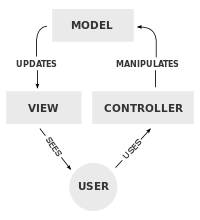
\includegraphics[width=0.5\textwidth]{model-view-controller}
 \caption{Model View Controller}
 \label{fig:model-view-controller}
\end{figure}

\subsubsection{Native Interface vs. Client Interface}

A native application interface is popular among server software and frequently used for desktop applications such as Microsoft Word and Microsoft PowerPoint, however, there has recently been a shift back to using a client, running back-end services in the cloud, exposing an API which can then be interacted with client side applications.

A separate client interface has multiple advantages and with modern networking speeds a user is typically unable to distinguish between running the interface on the server or a thin remote client \citep{schmidt1999interactive}.

The user is given the flexibility of using their preferred client to interface with the application, switching client without needing to worry about losing data, and developers are given the option to design a new interface without affecting the core application.

The user is also given the ability to interact with multiple instances of the application running remotely with no issues, which is particularly useful when running the application on a headless server.

Development of both the client and interface can also happen in parallel leading to better time to market in large development teams.

However, we must not forget the benefits of using a native application. By making the UI interface with the application over the network, a whole host of complexity and security issues arise. The development team needs to ensure that any user interacting with the API is authenticated and secure, as well as ensuring that there are no network issues between the interface and application.

The software itself also becomes more complex with a separate client as functionality needs to be built for handling network in both the UI and core application.

On balance, it makes sense for membrane to operate use a client interface. As Membrane will need to be run constantly, it needs to be able to operate as a software daemon. One of the requirements is to keep Membrane lightweight and maintenance free, running any user interface constantly would distract users.

Developers will also be able to build addition interfaces to Membrane if required, fulfilling the extensiblity requirement, and as both a GUI and CLI are required, this provides a nice way to develop both and gives users the desired flexibility between both.

\begin{figure}[t]
 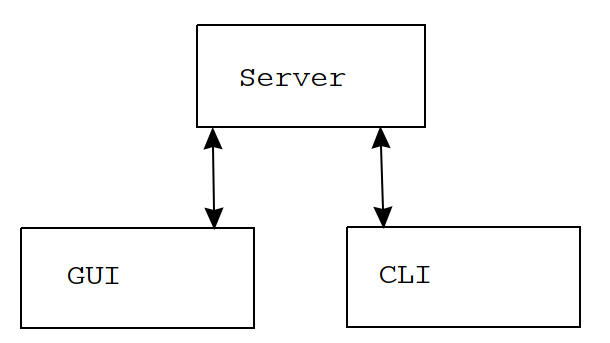
\includegraphics[width=0.5\textwidth]{client-server-model}
 \caption{Client Server Architecture}
 \label{fig:client-server}
\end{figure}

\subsubsection{Model View Controller (MVC)}

The Model View Controller (MVC) pattern, first described by \cite{krasner1988cookbook}, decouples the interface from the main logic of the program by establishing a subscribe notify protocol between them. The view must always reflect the state of the model and the model must always update the view when a change occurs.

This approach allows for code-reuse and lets the developer to create new models without rewriting the software, and provides high cohesion, meaning groups of related actions can be grouped together.

This has the disadvantage of making code harder to navigate due to added structural complexity, increasing scattering meaning multiple representations of objects need to be modified at the same time if required and increases the learning curve for developers, as they need to learn how to structure the application in a new way.

Although the MVC model provides a structurally sound way of building the application we need to generalise in into the N-Tier architecture for larger applications.

\subsubsection{N-Tier Architecture}

An N-Tier architecture is simply an extension of the MVC model, it takes the idea of layers in an application further, allowing sections of the software to be developed and tested without interfering with each other.

One of the key advantages to this approach is extra layers can be added and removed, even during run time. In Membrane we will look to take advantage of this when running in Tracker or Local Backup mode. The tracker can disable all of the local backup functionality, while the tracker only needs to run the network layer.

\begin{figure}[b!]
 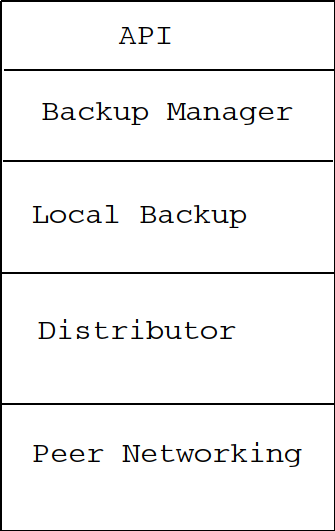
\includegraphics[width=0.5\textwidth]{membrane-n-tier}
 \caption{Membrane N-Tier Architecture}
 \label{fig:membrane-n-tier}
\end{figure}

We can see the Membrane N-Tier architecture in fig \ref{fig:membrane-n-tier}. Only modules next to each other are able to communicate directly and modules can be disabled as required.

The local backup performs all the basic tasks of file monitoring and local shard storage. The distributor monitors the local backup for shards to send to peers and packages them up to the Peer Networking layer for transmission. The Peer Networking layer is able to locate new peers and provides them to the Distributor if connected.

\section{Technologies}

The technologies used in a project can define the success of a software project. Incorrectly chosen tools can slow development and in some cases even cause projects to fail. While selecting technologies we will need to be weary of excitement surrounding modern technologies and look for unbiased advantages and disadvantages of each.

We will begin by selecting 

\subsection{Languages}

\subsection{Libraries}

\subsection{Frameworks}

\subsection{Tooling}

\chapter{System Components}

\section{Design}

\section{File System Monitoring}

\section{Local Storage System}

\section{Swarm Design}

\section{Peer Appraisal}

\chapter{User Interfaces}

\section{GUI}

\section{CLI}

\chapter{Results \& Evaluation}

\section{Unit Testing}

\section{Empirical Testing}

\section{Summary}

\chapter{Conclusion}

\section{Limitations}

\subsection{Limitations of the Study}

\subsection{Limitations of the System}

\section{Further Work}

\subsection{Expansion 1}

\subsection{Expansion 2}

\subsection{Expansion 3}

\section{Summary}

\bibliography{dissertation}

\end{document}
